\documentclass[uplatex,dvipdfmx,11pt,a4paper]{bxjsarticle}
\usepackage{amsmath,amssymb}
\usepackage{array}
\usepackage[dvipdfmx]{graphicx}
\usepackage{url}
\usepackage[haranoaji]{pxchfon}

\begin{document}

\begin{center}
{\LARGE \textbf{Transmission Theory Lesson4 Report}}
\end{center}

\vspace{1em}

\begin{flushright}
2611193 Heizo Nakai
\end{flushright}

\section*{STBCの送信ダイバーシティ利得の導出}

\subsection*{1. Alamouti符号}

送信する2つのシンボルを
\[
u_1,\ u_2
\]

とすると、送信は以下のように行われる。

\begin{center}
\begin{tabular}{c|c|c}
\hline
時刻 & アンテナ1 & アンテナ2 \\
\hline
$t_1$ & $u_1$ & $u_2$ \\
$t_2$ & $-u_2^*$ & $u_1^*$ \\
\hline
\end{tabular}
\end{center}

図\ref{fig:alamouti-stbc}に、授業資料で示されたAlamouti符号の送信系列と受信信号の関係を示す。

\begin{figure}[htbp]
\centering
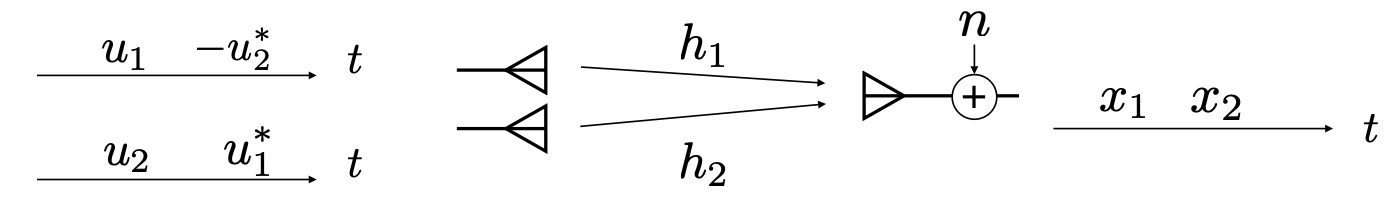
\includegraphics[width=0.95\linewidth]{figures/alamouti_stbc.png}
\caption{Alamouti符号における送信系列と受信構成（授業資料より引用）}
\label{fig:alamouti-stbc}
\end{figure}

受信信号は、

\[
x_1 = h_1u_1 + h_2u_2 + n_1
\]
\[
x_2 = -h_1u_2^* + h_2u_1^* + n_2
\]

となる。

これを行列表現すると、以下のようになる。

\[
\begin{bmatrix}
x_1 \\
x_2^*
\end{bmatrix}
=
\begin{bmatrix}
h_1 & h_2 \\
h_2^* & -h_1^*
\end{bmatrix}
\begin{bmatrix}
u_1 \\
u_2
\end{bmatrix}
+
\begin{bmatrix}
n_1 \\
n_2^*
\end{bmatrix}
\]

ここで、
\[
\mathbf{x}
=
\begin{bmatrix}
x_1 \\
x_2^*
\end{bmatrix},\quad
\mathbf{H}
=
\begin{bmatrix}
h_1 & h_2 \\
h_2^* & -h_1^*
\end{bmatrix},\quad
\mathbf{u}
=
\begin{bmatrix}
u_1 \\
u_2
\end{bmatrix},\quad
\mathbf{n}
=
\begin{bmatrix}
n_1 \\
n_2^*
\end{bmatrix}
\]

とおけば、
\[
\mathbf{x} = \mathbf{H}\mathbf{u} + \mathbf{n}
\]

となる。

\subsection*{2. 受信処理}

受信側ではチャネル行列のエルミート転置を掛ける。
\[
\begin{aligned}
\begin{bmatrix}
\tilde{u}_1 \\
\tilde{u}_2
\end{bmatrix}
&=
\mathbf{H}^{H}
\begin{bmatrix}
x_1 \\
x_2^*
\end{bmatrix} \\
&=
\mathbf{H}^{H}\left(\mathbf{H}\mathbf{u} + \mathbf{n}\right) \\
&=
\mathbf{H}^{H}\mathbf{H}\mathbf{u} + \mathbf{H}^{H}\mathbf{n} \\
&=
\left(\lvert h_1\rvert^2 + \lvert h_2\rvert^2\right)\mathbf{I}
\begin{bmatrix}
u_1 \\
u_2
\end{bmatrix}
+ \mathbf{H}^{H}
\begin{bmatrix}
n_1 \\
n_2^*
\end{bmatrix}
\end{aligned}
\]

ここで、$\mathbf{H}^{H}\mathbf{H}$ は以下のようになる。

\[
\mathbf{H}^{H}\mathbf{H}
=
\begin{bmatrix}
h_1^* & h_2 \\
h_2^* & -h_1
\end{bmatrix}
\begin{bmatrix}
h_1 & h_2 \\
h_2^* & -h_1^*
\end{bmatrix}
=
\left(\lvert h_1\rvert^2 + \lvert h_2\rvert^2\right)\mathbf{I}
\]

この結果、送信した2つのシンボルは互いに干渉することなく復元できる。

\subsection*{3. ダイバーシティ利得}

Alamouti符号を用いたSTBCでは、受信側で2つの送信シンボルを直交的に分離できる。
また、2本の送信アンテナを利用することで、受信側で得られる信号強度は
\[
\boxed{\lvert h_1\rvert^2 + \lvert h_2\rvert^2}
\]

となり、2つの独立した送信経路の信号強度が加算される。
したがって、一方のチャネルがフェージングによって弱くなっても、もう一方のチャネルによって受信品質を補うことができる。
このように、複数の独立した送信経路を利用することでフェージングに対する耐性が向上する効果を\textbf{送信ダイバーシティ利得}という。

\end{document}
